\documentclass[12pt,a4paper]{article} % Defines the document as an article with 12pt font on A4 paper
\usepackage[utf8]{inputenc} % Sets UTF-8 encoding
\usepackage{geometry} % Enables page geometry customization
\geometry{margin=1in} % Sets 1-inch margins
\usepackage{graphicx} % Allows inclusion of images
\usepackage{titlesec} % Controls section formatting
\usepackage{hyperref} % Enables hyperlinks
\usepackage{tikz}
\usepackage{amsmath}
\usetikzlibrary{shapes.geometric, calc, arrows.meta, positioning}
\usepackage{setspace} % Allows line spacing adjustments
\usepackage{csquotes} % Improves quotation handling
\usepackage{datetime} % Provides date and time formatting
\usepackage[backend=biber,style=apa, sorting=nyt]{biblatex} % Configures bibliography using Biber with APA style
\addbibresource{references.bib} % Adds a bibliography file (replace with your .bib file name)
\renewcommand{\dateseparator}{-} % Sets date separator as '-'
\onehalfspacing % Sets line spacing to 1.5


\title{\textbf{Research Proposal: PhD candidate in Industrial Engineering}} % Defines the title
\author{
	\textbf{Benjamin R. Berton}\\
	Polytechnique Montréal\\
	\href{mailto:benjamin.berton@polymtl.ca}{benjamin.berton@polymtl.ca}\\
	\textit{Supervised by: Philippe Doyon-Poulin}
} % Defines author details

\begin{document} % Begins the document
	\maketitle % Generates the title
	
	\begin{center}
		\textbf{A cognitive modelling approach to evaluating Human-Autonomy Teaming in commercial aviation}
	\end{center} % Centers the research title
	
	\begin{center}
		Submitted to members of the Jury:\\
		Pr. Jean-Marc Frayret, Pr. Philippe Doyon-Poulin \& Pr. Shi Cao\\
		\date{\today} % Inserts today's date
	\end{center} % Centers the research title
	
	\newpage % Starts a new page
	
	\tableofcontents % Generates the table of contents
	\newpage % Starts a new page
	
	\section{Trigger} % Defines a section titled "Trigger"
	Commercial aviation has shown a trend toward crew reduction, progressively decreasing the number of members in the cockpit \parencite{harris_human-centred_2007}. Historically, flight crews included up to five members, but technological advancements have reduced this number to two—the Captain (CPT) and First Officer (FO)—eliminating the need for flight engineers, navigators, and radio operators.
	
	Currently, the Federal Aviation Administration (FAA) - Part 25 regulations mandate a minimum of two pilots in the cockpit. However, technological advancements suggest the possibility of transitioning to Single Pilot Operations (SPO), where only one pilot would be on duty, assisted by advanced onboard technologies and potentially ground support \parencite{bilimoria_conceptual_2014}. While this transition is technically feasible, it introduces significant challenges, far more complex than previous crew reductions \parencite{matessa_using_2017}.
	
	One of the main issues with SPO is the removal of a redundancy layer, a fundamental element of aviation safety. Shifting from a two-pilot cockpit to a single-operator model requires ensuring an equivalent or higher level of safety compared to current operations \parencite{boy_requirements_2014}. Simply replacing the human co-pilot with increased automation is not a viable solution. Future operational concepts must rethink task distribution between the pilot and autonomy to maintain reliability and resilience.
	
	Successfully integrating SPO into commercial aviation requires moving beyond the traditional Human-Centered Design (HCD) approach. It is crucial to adopt a Human Systems Integration (HSI) perspective to ensure a seamless consideration of technical, organizational, and human dimensions throughout the system's lifecycle \parencite{boy_prodec_2024}. This transition will involve structural changes within air traffic management, raising new safety concerns. Identifying design flaws, anticipating potential human errors, and addressing them early in the development process are essential. The HSI approach allows for these aspects to be considered within a global operational framework, integrating interactions between human and technological elements.
	
	Another key factor for the success of SPO is the collaborative aspect between humans and advanced automated systems, known as Human-Autonomy Teaming (HAT). This approach emphasizes effective cooperation between the single pilot and advanced autonomous systems, where these systems do more than assist—they act as teammates \parencite{shively_autonomy_2017}.
	
	HAT is based on the evolution from automation to autonomy. Automation refers to technologies that process data, make decisions, and execute tasks based on predefined procedures \parencite{hoff_trust_2015, hancock_imposing_2017}. Autonomy, on the other hand, refers to a system’s ability to perform tasks with minimal human intervention over an extended period \parencite{endsley_here_2017, holbrook_enabling_2020}. This progressive shift toward greater autonomy fundamentally changes the human-automation relationship, evolving from simple interaction to genuine teamwork \parencite{endsley_here_2017}.
	
	However, increasing automation levels also presents challenges, particularly automation complacency, where excessive reliance on automated systems can lead to reduced vigilance and an inability to react effectively in case of anomalies \parencite{lee_design_2023}. To avoid this pitfall, it is crucial to design systems that promote active collaboration between the pilot and onboard autonomy \parencite{endsley_here_2017}. The goal of HAT is to ensure smooth and efficient cooperation, where autonomous systems act as real teammates, contributing to safer and more effective flight operations \parencite{mcneese_chapter_2020}.
	
	\section{Theoretical Background}
	\subsection{Human-Autonomy Teaming}
	\subsection{Situation Awareness}
	\subsubsection{Team-Situation Awareness}
	\subsubsection{Computational models of Situation Awareness}
	\subsection{Knowledge gap} % Section title "Knowledge Boundaries"
	
	%\section{Research Question and Hypothesis} % Section for research question and hypothesis
	%\textbf{Question:} How does introducing a virtual co-pilot based on a cognitive model influence pilot performance and situation %awareness in Single Pilot Operations?
	%
	%\textbf{Hypothesis:} A virtual co-pilot, designed with a rigorous cognitive model, improves pilot situation awareness while %reducing cognitive load.
	
	\section{Objectives} % Defines the "Objectives" section
	The general objective of this research is to develop a methodology that facilitates the design of an autonomous agent collaborating with a human pilot in commercial aviation operations. To do so, we will use a collection of methods from the human factors and ergonomics research toolkit, design an agent, and investigate how the design of the human-autonomy teamwork and agent interface impacts the team Situation Awareness.
	
	To achieve this objective, the thesis will be comprised of three phases. First, we will conduct a thorough analysis of the work and design domain in order to delineate the taskwork and teamwork and list requirements for the agent design. Second, we will develop in parallel a cognitive model of the human pilot and the autonomous agent, enabling them to interact in a closed-loop simulation environment. Third, we will conduct Human-In-The-Loop Simulation studies with expert pilots to both validate the cognitive model, and investigates the human factors that weren't modeled such as trust in the autonomous agent and usability of the interface. These phases will be detailed in the next section 
	
	\section{Methodology} % Section title "Methodology"
	\subsection{The use case scenario}
	The preliminary step for applying the methodology is to select a proper use case scenario, that is (1) realistic, so that information is easily available for modelling and knowledge gained can benefit the aviation industry, (2) challenging enough so that teaming with an autonomous agent is strongly beneficial for achieving good performance, and (3) procedural, deterministic, and short enough so that the cognitive modelling and agent implementation can be implemented inside Polytechnique's flight simulator platform.
	
	The scenario consists in a takeoff and initial climb phase with an engine failure due to a bird or drone strike. The scenario is performed by a single pilot in a multi-engine very light jet aircraft. Take-off with an engine failure is a challenging scenario for single pilot operations that is highly dynamic and require fast and precise decision-making from the captain. Bird and drone strike will be an issue for the foreseeable future of commercial aviation and is therefore a scenario of particular interest for the industry.

	\begin{figure}[h!]
 		\centering
  		\includegraphics[width=1\textwidth]{./images/scenario.png}
   		\caption{Takeoff scenario with a birdstrike causing an engine failure.}
		\label{fig:your-image-label}
	\end{figure}


	\subsection{Phase 1: Work and design domain analysis}
	The first step of the methodology involves analyzing the current state of commercial aviation operations to understand the design domain of the to-be-designed Autonomous Agent (AA). Two complementary methods are used, the Goal Directed Task Analysis (GDTA) and the Interdependence Analysis (IA).

	\subsubsection{Goal-Directed Task Analysis}
	A GDTA was conducted to understand the information needs inherent to commercial aviation operations. GDTA is a task analysis methodology aimed at identifying the critical information human operators must acquire and process to achieve their mission goals effectively and safely. This information contributes to the construction and maintenance of Situation Awareness (SA), a key predictor of operational performance and safety in commercial aviation \parencite{endsley_here_2017}. %Verify this ref, goal is to say SA is predictor of operational performance. SotA on SA might be good
	Following the established GDTA outlined by Endsley and Jones for a complete commercial aviation flight \parencite{endsley_designing_2003}, our GDTA was constructed by selecting the relevant hierarchy of goals and associated information requirements for our takeoff scenario. To enrich and validate the GDTA, four experienced commercial pilots were recruited and interviewed. Their insights were incorporated to ensure that the analysis reflects the operational realities of contemporary flight environments.

	The GDTA resulted in a hierarchically organized representation of pilot goals, each associated with the specific information necessary for optimal task performance. This structured output serves as a foundation for designing the human-autonomy team. Specifically, the identified information elements will guide the development of the Autonomous Agent, ensuring that both the human pilot and the synthetic teammate maintain a sufficient level of SA throughout the operation.

	The goal is to ensure that the closely coupled human-agent team maintains alignment of their respective situation representation by attending both to the proper information for the task at hand. This alignment supports the development of Team Situation Awareness (Team SA)—the state in which each teammate possesses an accurate understanding of the situation relevant to their roles within the flight deck.
	This notion is visually represented by Figure~\ref{fig:team-sa-venn}, where individual SA of each team member contributes to the larger construct of Team SA. Furthermore, a significant overlap in individual SA defines the concept of Shared Situation Awareness. Achieving and maintaining both individual SA and shared SA between the human and autonomous teammate is critical to ensuring coordinated, safe, and effective operations.

	\begin{figure}[h!]
		\centering
		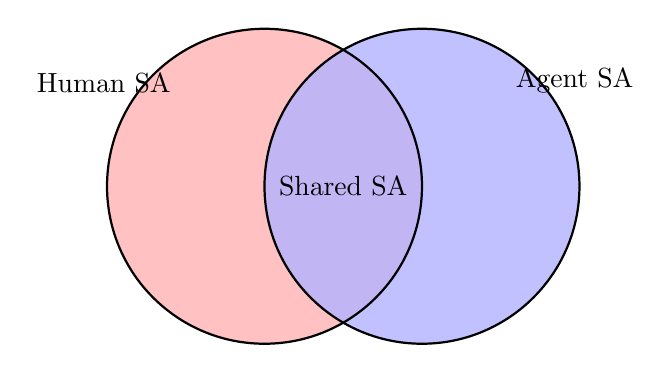
\begin{tikzpicture}
        % Left circle (Human SA)
        \fill[red!30, opacity=0.8] (-1,0) circle (2);
        % Right circle (Agent SA)
        \fill[blue!30, opacity=0.8] (1,0) circle (2);

        % Borders
        \draw[thick] (-1,0) circle (2) node[above left=1.5cm] {Human SA};
        \draw[thick] (1,0) circle (2) node[above right=1.5cm] {Agent SA};

        % Label overlap
        \node at (0,0) {Shared SA};
		\end{tikzpicture}
		\caption{Venn diagram illustrating Team Situation Awareness (Team SA) with the overlapping individual SA of the human pilot and the autonomous agent representing Shared SA.}
		\label{fig:team-sa-venn}
	\end{figure}

	\subsubsection{Interdependence Analysis}
	Interdependent Analysis is a work analysis methods part of the coactive design process that helps improve collaboration between humans and machines by identifying key interdependence relationships that are essential for effective teamwork \parencite{johnson_coactive_2014}. It also defines the requirements for tasks that involve interdependence, ensuring successful cooperation. This framework consists of three main parts: (1) joint activity modeling, (2) interdependence assessment, and (3) workflow analysis. These components help guide the design of systems for more effective teamwork, particularly in human-autonomy teams \parencite{johnson_understanding_2018}.
	To define human and autonomy role for our case study we have performed an Interdependence Analysis. This tool's most powerful feature is its ability to map different teaming options at the beginning of the design process, as opposed to a single function allocation solution. The output of an IA gives:
	\begin{itemize}
		\item Different teaming alternatives, especially in our case the dyad human-agent with human as main performer of the activity and agent as supporter or conversely agent as the main performer and human as the supporter.
		\item A visualization of possible workflows for the team to carry-out the activity, depending on the team alternative, required, and opportunistic interdependence relationship.
		\item A list of \textbf{Observability, Predictability, and Directability} requirements to ensure proper collaboration for the human-autonomy team.
	\end{itemize}
	The output of the GDTA was used to facilitates the IA, the goal hierarchy served to create the Joint Activity Graph, which is a hierarchical task decomposition of the activity, and the information requirements also guided the fine-level task definition.
	\subsection{Phase 2: Cognitive modeling and agent development}

	\begin{figure}[h!]
		\centering
		% First logo
		\begin{minipage}[b]{0.3\textwidth}
			\centering
			\raisebox{2mm}{\includegraphics[width=0.9\textwidth]{images/hierarchy_diagram.png}}
		\end{minipage}
		% Second logo
		\begin{minipage}[b]{0.3\textwidth}
			\centering
			\includegraphics[width=0.6\textwidth]{images/workflow_icon.png}
		\end{minipage}
		% Third logo
		\begin{minipage}[b]{0.3\textwidth}
			\centering
			\includegraphics[width=0.8\textwidth]{images/requirements.png}
		\end{minipage}
		\caption{Output of phase 1 - goal hierarchy, task workflow, information \& OPD requirements.}
		\label{fig:logos}
	\end{figure}
	The phase 1 allowed us to delineate the design domain and list detailed information as well as teaming requirements that will be useful for the modelling and agent design phase.
	\begin{itemize}
		\item The goal hierarchy will be used for the task structure of the cognitive model and the agent, each goal from the GDTA will be implemented in the cognitive model using the goal module of the ACT-R architecture, responsible for holding the current goal or focus of attention of the model. Likewise, agent-side, the goal hierarchy will be represented as a structure containing states and transitions akin to a Finite State Machine (FSM)
		\item Workflows from the IA will be used as an input to a module responsible for the task allocation between the model and the agent, for each workflow, this "dispatcher" module will effectively activate or inhibit actions for the model and agent.
		\item Information requirements will be used to program that both the model and agent attend to the relevant elements of the environment for the task at hand. It will also be used for Team Situation Awareness assessment, as the cognitive model can be asked to answer questions regarding the value/status of relevant information for the task, and information representation of the agent can be inspected at any time, thus the alignment in situation representation can be approximated by the difference in situation representation for both teammates. OPD requirements will be individually assessed during simulation by observing team behavior.
	\end{itemize}

	\subsubsection{QN-ACTR and SEEV}
	The cognitive model of the single pilot will be implemented using the QN-ACTR architecture, integrating a simplified SEEV model to capture attention allocation dynamics and level 1 situation awareness (SA). Based on the output from Phase 1 (interdependence analysis), operational documentation, and available training materials, an initial model of an expert pilot operating a Cessna Citation Mustang will be developed. The model will simulate routine decision-making and procedural execution, following Standard Operating Procedures (SOPs) and checklists for the takeoff phase, witout any assistance from an autonomous agent.

	The model will be connected to X-Plane 11 in a closed-loop simulation, receiving real-time aircraft and environment data via bidirectional UDP and issuing control inputs directly to the simulator. Once validated in this baseline condition, the model will be extended to collaborate with the autonomous agent, enabling the pilot model to observe and direct the agent's actions, again via UDP.
	
	The model will be implemented in Lisp and integrated into the QN-ACTR platform, with necessary adjustments to the platform to ensure appropriate input/output handling with X-Plane 11. Development will build upon the QN-ACTR takeoff model by Xu et al. \parencite{xu_modeling_2021}, which currently models a single-pilot normal takeoff procedure in a Cessna 172 aircraft.
	
	The SEEV model will be applied to determine the probability of the pilot allocating attention to relevant Areas of Interest (AOIs) in the cockpit and external environment. The SEEV parameters—Salience, Effort, Expectancy, and Value—will initially adopt the coefficient weights proposed by Wang et al. \parencite{wang_real-time_2024}, whose model was tuned for a similar scenario (engine failure at takeoff in Single Pilot Operations). Their configuration defines seven AOIs: (1) Primary Flight Display (PFD), (2) Navigation Display (ND), (3) Engine/Warning Display (E/WD), (4) System Display (SD), (5) Central Console, (6) Flight Manual, and (7) Outside Window.
	
	The attention probability ($P(AOI)$) towards each AOI will be computed using a simplified version of SEEV, where Effort and Salience parameters are discounted, following common practices in driving and aviation simulator studies \parencite{}. This is justified by the reduced visual angles and minimal scanning effort required in such setups. The attention allocation formula is defined in Equation~\ref{eq:VA_AOI}:
	
	\begin{equation}
		VA_{AOI} = \sum_{t=1}^{n} (Ex_t) (R_t) (P_t)
		\label{eq:VA_AOI}
		\end{equation}
	Here, $VA_{AOI}$ is the raw attention value for an AOI, $t$ indexes across $n$ tasks, $Ex_t$ is the Expectancy of the AOI for task $t$, $R_t$ is its Relevance, and $P_t$ is the Priority of task $t$. The combined effect of $R_t$ and $P_t$ represents the "Value" factor in the SEEV framework.
	
	The resulting $VA_{AOI}$ values are normalized to generate probabilistic attention weights across all AOIs. Monte Carlo simulations will be used to stochastically determine gaze allocation over time.
	
	The model thus accounts for both attentional and memory constraints: attention allocation drives what information enters the cognitive system, while ACT-R's declarative memory mechanisms (e.g., memory decay and activation thresholds) govern subsequent retention and retrieval. In QN-ACTR, activation levels of chunks representing critical elements must exceed a threshold to contribute to Level 1 SA (perception-based SA). Consequently, Level 1 SA in this model emerges from the interaction between visual attention (SEEV) and cognitive memory dynamics (ACT-R). The framework is presented in Figure~\ref{fig:qn-actr-seev}

	\begin{figure}[h!]
    \centering
    \includegraphics[width=0.9\textwidth]{./images/qn-actr-sa-synoptic.png}
    \caption{Overview of the QN-ACTR-SEEV framework. Stages 1-3 (marked on the lines in the figure) signify the different cognitive processes necessary in the acquisition and maintenance of Level 1 SA. Adapted from Rehman (2020) \parencite{rehman_phd_thesis}.}
    \label{fig:qn-actr-seev}
	\end{figure}


	%this is from umair thesis and need to be modified and cited


	\subsubsection{Agent design}
	A functional prototype of the Autonomous Agent (AA) system will be developed in parallel with the cognitive model to meet the previously defined requirements. The prototype will be deployed as a tablet application interfacing with the flight simulator and positioned within the cockpit environment.

	The AA is implemented as a modular and reactive software component designed to assist the pilot in managing the flight scenario. The agent adopts a nested Finite State Machine (FSM) architecture, employing the state pattern, to organize its behavior into a structured hierarchy of states and substates. Each state encapsulates a specific procedural phase of the scenario, with transitions triggered by defined environmental conditions.
	
	This design was selected to reflect the deterministic and highly procedural characteristics of the flight scenario. The agent does not incorporate deliberative planning or uncertainty handling; rather, it functions as a partial Wizard of Oz system. Its purpose is to emulate the expert-like behavior of an AI system that executes preprogrammed actions in response to situational cues.
	
	The AA system is composed of the following modules: \begin{itemize} \item \textbf{State Hierarchy:} A layered structure of states and nested substates representing sequential and conditional phases of the flight (e.g., "Takeoff Roll" $\rightarrow$ "Bird Strike Response" $\rightarrow$ "Post-Incident Assessment"). \item \textbf{State Manager:} A supervisory module responsible for managing transitions between states based on predefined transition rules. \item \textbf{Action Layer:} A set of atomic actions (e.g., "Verify engine instruments", "Declare emergency to ATC") executed when specific states or substates become active. \item \textbf{Status Monitoring:} A continuous input channel from the flight simulator (X-Plane 11) used to assess scenario conditions and update the agent's internal state. \end{itemize}
	
	The nested FSM structure provides a modular and scalable framework, ensuring ease of maintenance and facilitating the alignment between the agent's reactive behavior and the cognitive model's procedural logic.

	\begin{figure}[h!]
		\centering
		\includegraphics[width=1.0\textwidth]{./images/AA_synoptic.png}
		\caption{AA Synoptic diagram}
		\label{fig:aa_synoptic}
	\end{figure}
	
	\subsubsection{System architecture}
	The whole system architecture consists of three principal components: the Cognitive Model (QN-ACTR + SEEV), the AA, and the Task Dispatcher. These components operate within the same local network.

	\begin{itemize} \item \textbf{Task Dispatcher:} A central module responsible for allocating tasks between the cognitive model (representing the human pilot) and the AA (the virtual copilot). The dispatcher can be thought of representing the Human-Autonomy pre-flight briefing. It activates or inhibit tasks for each member of the team, ensuring overall coherence between entities for effective collaboration to achieve the shared set of goals. \item \textbf{Cognitive Model:} The QN-ACTR+SEEV model simulates the pilot's cognitive processes, including level 1 situation awareness, memory dynamics, and attention allocation. It is capable of both executing tasks directly and interacting with the AA. \item \textbf{Autonomous Agent (AA):} As outlined earlier, this agent handles delegated tasks from the dispatcher and takes direct action in the simulation environment to assist the pilot. \end{itemize}

	The system leverages the \textbf{Ingescape ecosystem} to connect distributed modules seamlessly: \begin{itemize} \item \textbf{Black-box agents:} Each software module (dispatcher, cognitive model, AA agent) is implemented as an independent black box with defined input/output ports. \item \textbf{ZeroMQ-based messaging:} Ingescape abstracts communication, enabling asynchronous and decoupled messaging between components. \item \textbf{Simulation Interface:} Both the AA agent and the cognitive model exchange real-time data with X-Plane 11 and between themselves, ensuring they operate with a synchronized and shared representation of the environment. \end{itemize}

	This architecture enables flexible experimentation, including various teaming strategies (e.g., autonomous agent as backup or co-pilot), and modular upgrades to individual system components.

	\subsubsection{Scenario \& Simulation}
	\subsection{Phase 3: Human-In-The-loop simulation studies}
	\subsubsection{Scenario}
	\subsubsection{Equipment}
	\subsubsection{Participants}
	\subsubsection{Protocol}
	\subsubsection{Model validation and results}
	
	\section{Expected Results} % Section for expected results
	\begin{itemize}
		\item A cognitive model predicting pilot cognitive load and situation awareness.
		\item An evaluation of human-autonomy cooperation strategies.
		\item Empirical validation via HITLS to assess acceptance of the autonomous co-pilot.
	\end{itemize} % Lists expected outcomes
	
	\section{Originality and Impact} % Section for originality and impact
	This project provides an advanced methodology for integrating collaborative autonomous systems into the cockpit, improving the safety and efficiency of Single Pilot Operations.
	
	\section{Risks assessment and mitigation}
	My risks
	
	\section{Resource management}
	My resources
	
	\section{Timeline}
	\printbibliography % Prints the bibliography
	
\end{document} % Ends the document
